\section{Arquitetura de sistema}

A arquitetura do sistema desenvolvido pela equipe Oshkosh pertence a classe de
arquitetura de camadas, onde cada camada depende dos dados das camadas
inferiores, não das superiores. Apesar de citado como característica comum
em sistemas de camadas, no artigo do grupo \citep{chen2009terramax}, as
dependências não necessariamente são de cima para baixo. A arquitetura de três
camadas, estado da arte das arquiteturas robóticas, utilizada por diversos
sistemas autônomos, como o AUV Phoenix \citep{gat1991reliable} e o veículo
Stanley \citep{montemerlo2006winning}, pode possuir dependências no estilo
``top-down'' ou interdependência entre camadas.

Essa arquitetura apresenta a grande vantagem de ser flexível e
modular, já que o desenvolvimento de cada camada não depende das outras e as
dependências podem ser simuladas através de objetos \textit{mock}. Com isso,
cada equipe pode trabalhar em sua especialidade, otimizando o tempo e
aumentando a qualidade dos algoritmos desenvolvidos em cada função. Vale
ressaltar que, ao fim do desenvolvimento de cada subsistema, o sistema deverá
ser integrado, portanto o protocolo de comunicação entre camadas e a
plataforma/framework de integração é crucial nesse tipo de arquitetura.

São apresentados sete sistemas~\ref{fig:camadas}: 
   
\begin{enumerate}
  \item \textit{System Control and User Interface} - normalmente encontrado na
  literatura como \textit{Mission Control System}, ou planejamento de
missão (\textit{Mission Planning}) ou planejamento de tarefas (\textit{Task
Planning}). Como definido em \cite{fryxell1996navigation}, o controle de
missão é um sistema que permite ao operador definir as missões de um veículo em
linguagem de alto nível, provê ferramentas adequadas para converter planos em
Programas de Missões que podem ser verificados e executados em tempo real, e
permite ao operador saber o estado da missão enquanto esta é executada, e
modificá-la se for necessário.

  \item \textit{Autonomous Behavior} - é a parte que compõe a autonomia do robô,
  responsável pelo planejamento de trajetórias, e gerenciamento dos
  comportamentos do robô.
  
  \item \textit{Vehicle Management} - camada com os algoritmos de controle
  (controle de posição, estabilidade, velocidade,e  outros).
  
  \item \textit{Perception} - camada que possui os algoritmos de percepção, como
  detecção de obstáculos, detecção da via, detecção de tráfego, detecção de
  faixas, e outros.
  
  \item \textit{Sensor} - \textit{drivers} de sensores, usados para os
  algoritmos de percepção, como câmeras, LIDAR, e outros.
  
  \item \textit{Vehicle Status and Navigation} - sensores para o sistema de
  controle, como posição, velocidade, aceleração e estado do veículo.
\end{enumerate}
 
\begin{figure}[!ht]
\centering
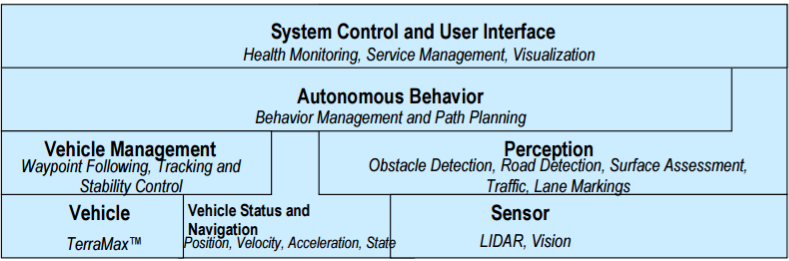
\includegraphics[width=\columnwidth]{figs/camadas.jpg}
\caption{Arquitetura de camadas do veículo TerraMax}
\label{fig:camadas}
\end{figure}

O autor não se aprofunda, no artigo, em como é realizada a integração entre as
camadas, isto é, como a informação e dados transitam, porém ele utiliza
uma terminologia comumente presente na literatura: ``serviços'' e
``\textit{publisher-subscriber}''. Frameworks como o ROS, estado da arte,
possibilitam a utilização de ambos os tipos de comunicação.

\begin{itemize}
  \item \textit{serviço ou cliente-servido} -  componentes falam diretamente
  com outros componentes. As vantagens deste protocolo são: definição prévia da
  interface; e é uma abordagem distribuída para comunicação, já que não há um
  módulo central que distribui os dados. Uma desvantagem deste protocolo é o
  \textit{overhead}, que é significativo se muitos componentes precisam de uma
  mesma informação.
  
  \item \textit{publish-subscriber} - um componente publica dados e qualquer outro componente
pode subscrever (ouvir) a esse dado. Normalmente, há um processo central que
roteia os dados entre \textit{publish} e \textit{subscriber}. Em uma arquitetura
típica, um componente pode publicar e subscrever a vários tipos de informações.
As vantagens desse protocolo de comunicação são: simplicidade e pouco
\textit{overhead}; ideal quando não se sabe quantos componentes diferentes
necessitarão dos dados (como em muitas interfaces); componentes não ficam
sobrecarregados em caso de múltiplos pedidos de um mesmo dado. Suas principais
desvantagens são: difícil depuração de código, pois normalemente a sintaxe da
mensagem está escondida em uma simples \textit{string} (uma \textit{lista}
pode ser enviado como \textit{string} e o componente subscritor retraduz);
utilização de um servidor central que distribui as mensagens (recebe dos
\textit{publishers} e envia aos \textit{subscribers}), o que pode criar um único
ponto de falha e sobrecarga.
   
\end{itemize}

As camadas de \textit{System Control and User Interface} e \textit{Autonomous
Behavior} se comunicam através de mensagens do tipo serviço, enquanto que os
dados da camada \textit{Sensor} são publicados para as demais camadas.

\subsection{Autonomous Behavior}

A camada do sistema autônomo é desenvolvida no componente de software chamado
\textit{Autonomous Vehicle Manager} (AVM), cujos blocos de software estão
detalhados na Fig.~\ref{fig:avm}. 

\begin{figure}[!ht]
\centering
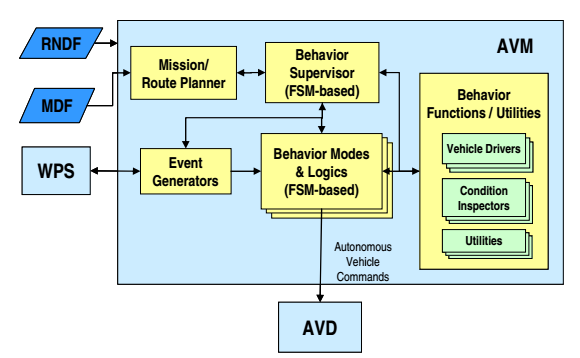
\includegraphics[width=\columnwidth]{figs/AVM}
\caption{Blocos funcionais do \textit{Autonomous Vehicle Manager}}
\label{fig:avm}
\end{figure}

As funcionalidades de cada bloco são:

\begin{itemize}
  \item Mission Behavior Supervisor (MBS): gerencia e avalia o estado
  da missão (objetivos e subobjetivos), seleciona e supeervisa os modos de comportamento apropriados
  para a execução;
  \item Mission Route Planner: gera rotas e planos de alto nível baseado nos
  segmentos de rota disponibilizados e zonas definidas no Road Network
  Definition File (RNDF), um arquivo disponível a todos os participantes do
  desafio, o qual contém o mapa e trechos a serem percorridos;
  \item Behavior Modes \& Logic: contém um conjunto de modos de comportamento,
  suas relações de transição e lógica de execução;
  \item Event Generators: monitora o veículo e estima o estado do ambiente pelos
  dados do WPS (dados dos sensores processados), gerando eventos apropriados
  para os modos comportamentais quando há mudanças abruptas (e.g. obstáculos);
  \item Behavior functions/utilities: provê serviços comuns para os
  comportamentos, como geração de trajetórias e etc.
\end{itemize}

\subsubsection{Behavior Supervisor e Behavior Modes}

O controle supervisório adotado pelo grupo Terramax é baseado em um sistema de
evento discreto com Máquinas de Estado Finito (\textit{Finite State Machine},
FSM) para gerar e executar os comportamentos do veículo. Observou-se que FSM é
uma solução simples para solucionar o desafio e modela, de forma eficiente, as
regras/restrições e comportamentos/táticas do robô. Vale observar que esta é uma
estrutura hierárquica, estruturada e rígida, de forma que não é a arquitetura
ideal para ambientes extremamente dinâmicos, como é o caso da via urbana. 

Apesar de usar a terminologia e ideologia de modelagem do robô em
comportamentos, a arquitetura desenvolvida não é uma arquitetura baseada em
comportamentos (Arquitetura Reativa), como aquela apresentada por
Arkin~\cite{arkin1998behavior}. Tampouco Terramax é uma Arquitetura
Híbrida, já que o Behavior Supervisor desempenha um papel centralizador, o que 
caracteriza sua arquitetura como Deliberativa.

Foram criados dezessete modos comportamentais: ChangeLane, DriveInLane,
DriveInZone, DriveToTarget, Emergent Drive, ExitParkingSpot,
InspectIntersection, InspectLaneTurn, InspectPassing, InspectUTurn,
InspectZoneIntersection, Park, Pass, PassRecovery, PerformUTurn,
RoadBlockRecovery e Wait., todos modelados como máquinas de estado finito
com parâmetros (FSMwP). Uma missão pode corresponder a um conjunto de
comportamentos, conectados logimcamente, também com FSMwP. Essa conexão entre
comportamentos para executar uma missão foi chamado de Mode Transition Machine
(MTM) e corresponde a um modelo estrutural usado pelo Behavior Supervisor para a
supervisão, cuja teoria foi desenvolvida em~\cite{chen2001safety}.

Como foi comentado pelo próprio autor, o modelo de FSMwP funciona de maneira
intuitiva para a geração dos comportamentos e lógica de transição, porém sofre
dos mesmos problemas de uma arquitetura deliberativa, ou seja, robustez a
situações inesperadas e a falta de soluções criativas para a solução de
problemas, já que tudo é ``scripted''.

A fim de exemplificar esse problema, suponha que o Terramax observe um carro
lento a frente e entre no modo de ultrapassagem. O comportamento de
ultrapassagem é a combinação dos comportamentos ``Troca de faixa", ``Dirigir
em frente", até a ultrapassagem do veículo, e ``Troca de faixa" novamente. Se
houver, porém, um segundo veículo, logo a frente do primeiro, impedindo a
segunda ``Troca de faixa'', o Terramax terá que entrar em um sistema de
recuperação de falhas, já que este evento não havia sido pré-codificado. Observe
que há outras diversas combinações de eventos a serem considerados, o que se
torna impossível em uma arquitetura hierárquica rígida.

\subsubsection{Route planning e Trajectory planning}

O componente de software que realiza o Route Planning do veículo Terramax tem
por objetivo gerar uma lista ordenada dos segmentos definidos no arquivo RNDF, o
que possibilita ao veículo visitar os \textit{checkpoints} desejados, em
sequência. Os segmentos do RNDF e \textit{checkpoints} foram modelados como um
grafo, Fig.~\ref{fig:route}. O melhor caminho é computado a partir do método de
busca gulosa Dijkstra, bem conhecido na literatura \cite{cormen2001dijkstra}. O
tempo de viagem estimado foi utilizado como função custo para o método, em vez
da distância entre segmento. Essa modificação mostrou maior eficiência durante a
execução, pois levou em consideração limite de velocidade da via, condições do
tráfego, e possíveis obstáculos.

\begin{figure}[!ht]
\centering
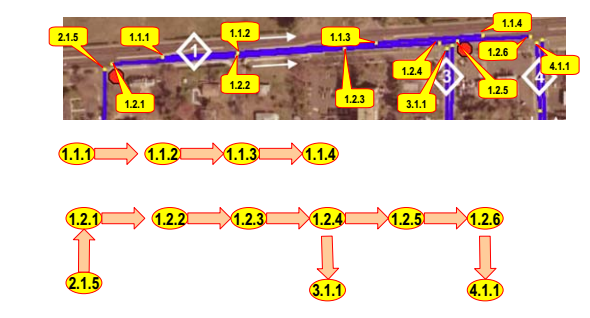
\includegraphics[width=\columnwidth]{figs/route}
\caption{Route planning modelado como um grafo de segmentos.}
\label{fig:route}
\end{figure}

Após o cálculo da melhor rota, transição dos segmentos computada pelo método de
Dijkstra, o planejador de trajetórias gera uma sequência densa e viável de
pontos objetivo (posição, \textit{waypoints}) dentro de cada segmento, com suas
correspondentes velocidades objetivo. O controle de velocidade e posição é
realizado pelo componente de software AVD (\textit{Vehicle Status and
Navigation}), a camada funcional da arquitetura. 

Foram desenvolvidos quatro tipos de \textit{trajectory planner}, os quais são
utilizados dependendo da situação em que o veículo se encontra:

\begin{itemize}
  \item \textit{Lane-following trajectory planner}: utiliza os sensores para
  detectar as bordas (meio-fio) e gera pontos objetivo no centro da via. A
  velocidade alvo é determinada considerando o espaço entre o TerraMax e o
  veículo em frente, a dinâmica do robô (e.g. velocidade atual,
  aceleração e desaceleração limite), e limite de velocidade da via.
  \item \textit{Template-base trajecotyr planners}: é um conjunto de
  planejadores que podem gerar rapidamente pontos objetivo usando padrões
  instanciados. É comum em manobras padronizadas, como troca de faixa, rotar em
  interseções e outros. 
  \item \textit{Open-space trajectory planner}: provê a geração de trajetórias e
  desvio de obstáculos em um espaço aberto, isto é, ausência de via. Foi adotado
  um algoritmo similar com o A* (ou Dijkstra) após a discretização do espaço.
\end{itemize}

Os planejadores de rota e trajetória são semelhantes aos utilizados por outros
veículos do desafio e utilizam algoritmos bem consolidados na literatura. 
